\subsection{Face recognition}
\IEEEPARstart{T}{he} need to identify people can be split into two distinct areas based on the diversity of the requirements that are typical to each area: these are Law Enforcement and Civilian application areas.

\subsubsection{Civilian applications }

Most are used to verify the identity of a person, the aim being to allow him or deny certain privileges. Thus, these applications are used to identify a large number of people in real time. They are fast and accurate because the reference image has a good quality and image control is taken from the front in optimal conditions.
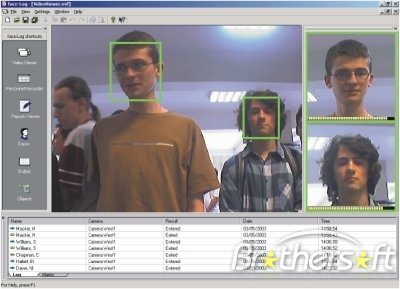
\includegraphics[width=\linewidth]{img/face_recognition_civil}
Exemples of civilian applications : Passport verification at the airport, windows logon, access to a secure area 

\subsubsection{Law applications }
In the police, some needs are similar to those of the civilian sector, but there are other cases such as the identification of a suspect filmed by a CCTV camera where conditions are less optimal.
The image is often of poor quality, not always face, facial expression is not neutral, the brightness is different reference pictures.
Again, this time the comparison is not with a single image but with a whole database. The work to be done quickly became much more consistent.

The table~\cite{NPIA} below shows the similarity between the fingerprints searching and the face recognition.

~\\
\begin{tabular}{|p{0.28\linewidth}|p{0.28\linewidth}|p{0.28\linewidth}|}
\hline
\textbf{Fingerprints searching}&\textbf{Face Recognition}&\textbf{Capability}\\
\hline
Ten print to Ten print searching&Mugshot to Mugshot&Identification of an Live Image to Mugshot individual in custody\\
\hline
Ten print to Mark searching&Mugshot to CCTV image&Linking known individuals to unsolved crimes\\
\hline
Mark to Ten print searching&CCTV image to Mugshot&Identifying suspects from forensic evidence at crime scenes\\
\hline
Mark to Mark&CCTV images from multiple cameras&Linking unsolved crimes together\\
\hline
\end{tabular}

~\\
\subsubsection{What are the difficulties ? }
\subsubsection{How does it work ? }

\subsection{Face expression recognition}

